\documentclass{article}

% Language setting
% Replace `english' with e.g. `spanish' to change the document language
\usepackage[portuguese]{babel}

% Set page size and margins
% Replace `letterpaper' with `a4paper' for UK/EU standard size
\usepackage[a4paper,top=2cm,bottom=2cm,left=3cm,right=3cm,marginparwidth=1.75cm]{geometry}

% Useful packages
\usepackage{amsmath}
\usepackage{subcaption}
\usepackage{graphicx}
\usepackage[colorlinks=true, allcolors=blue]{hyperref}

\title{Trabalho Prático 04}
\author{Luciano Stork}

\begin{document}
\maketitle

\begin{abstract}
A utilização das técnicas de codificação de Huffman e Shannon-Fano desempenha um papel essencial na compressão de dados, com o propósito de reduzir o volume das informações sem comprometer a sua qualidade. A aplicação destas técnicas a imagens no formato PNM envolve a representação eficiente dos valores dos pixels, sendo esse um aspecto fundamental para otimizar o espaço de armazenamento e a transmissão de imagens. Adicionalmente, a codificação da diferença móvel entre pixels assume uma importância significativa na otimização da transmissão de imagens e vídeos. Ao codificar apenas as variações entre os valores dos pixels sucessivos, em vez de lidar com valores absolutos, é possível economizar recursos de largura de banda e espaço de armazenamento de maneira eficiente. 

Neste projeto acadêmico, foram implementados algoritmos de codificação de Huffman e Shannon-Fano aplicados à imagens PNM. Além disso, foram desenvolvidos métodos eficazes para codificar as diferenças móveis entre os pixels, o que tornou possível de capturar e representar de maneira precisa as variações nos valores das unidades básicas dos quadros consecutivos de imagens. A combinação dessas técnicas e análises de codificação não apenas desempenha um papel crucial na eficiência da transmissão de imagens e vídeos, 
 economizando largura de banda e espaço de armazenamento; mas também tem impacto substancial na evolução de soluções tecnológicas avançadas. Tal compressão de dados proporcionada por essas técnicas reflete em avanços tangíveis que impulsionam a eficiência e a acessibilidade de aplicações tecnológicas, tornando-se essenciais para o cenário das telecomunicações e processamento de imagens.

\end{abstract}

\section{Implementação do algoritmo}
\subsection{Preparação}

Para iniciar, de fato, a implementação do código, é interessante conhecer qual é a natureza do objeto-base da aplicação. Sendo assim, cito que uma imagem PNM, ou "Portable Any Map," é um formato de arquivo de imagem versátil que pode representar imagens em preto e branco, tons de cinza ou colorida. Sua característica mais distintiva é a representação textual completa, o que a torna facilmente legível e editável por humanos justamente por não apresentar, em essência, nenhum tipo de compactação. Dessa forma, é uma escolha assertiva considerar a utilização desse formato para lidar com métodos de compactação de dados nos moldes da Teoria da Informação e da Codificação, já que o formato explorado mantém todas as informações originais da imagem sem perdas de qualidade, contribuindo para uma base clara e íntegra para demonstrar os efeitos das técnicas de compactação.

Considerei, para análise e aplicação das consequentes codificações diferentes imagens, obtida via Web. A nível de informação, trata-se de figuras com diferentes tamanhos. Adiante, irei explorar as implicações dessa informação no desempenho do scrip Matlab desenvolvido.

\subsection{Codificação de Huffman aplicada à imagem PNM}

Com o crescimento da quantidade de dados gerados e
transmitidos, é interessante pensar em formas de otimização dessas transmissões de modo a garantir, por exemplo, a não sobrecarga da rede. A compactação, portanto, torna-se cada dia mais essencial, economizando largura de banda em transmissões de dados e reduzindo o espaço necessário para armazenar informações, o que é fundamental em um mundo cada vez mais digital e conectado.

Existem várias técnicas que visam compactar dados, sendo a mais comum as abordagens que adequam o número de bits usados para representar os caracteres mais frequentes. Pensando nisso, a \textbf{Codificação de Huffman} é uma técnica de compactação de dados que se concentra na redução do tamanho de arquivos armazenados nos mais diversos formatos. Ela opera calculando uma tabela de códigos personalizada para o arquivo original, atribuindo códigos de comprimento variável para cada caractere ou símbolo com base em sua frequência de ocorrência. Isso significa que os caracteres mais comuns receberão códigos mais curtos, enquanto os menos frequentes terão códigos mais longos. A grande vantagem desse método é que ele resulta em uma representação altamente eficiente do arquivo original, economizando espaço de armazenamento ou largura de banda durante a transmissão. Essa codificação é amplamente usada em telecomunicações e na compactação de arquivos em geral, tornando-se uma ferramenta essencial em sistemas de comunicação e armazenamento de dados.

Analisando a biblioteca do Matlab, encontro três comandos que basicamente atenderão a tarefa de compactar e descompactar o objeto em análise, sendo eles o \textbf{huffmandict}, \textbf{huffmanenco} e o \textbf{huffmandeco}:

\begin{itemize}
\item Iniciando com o comando \textbf{huffmandict}, esta função desempenha o papel de criar um dicionário de Huffman. Esse dicionário é uma espécie de "mapa" que associa símbolos aos seus códigos de Huffman correspondentes, com base na frequência de ocorrência desses símbolos nos dados. A ideia principal é que símbolos mais comuns recebem códigos mais curtos, enquanto os menos comuns são representados por códigos mais longos. Esse dicionário funciona como uma tabela de referência fundamental para os processos subsequentes de codificação e decodificação, já que determina como cada símbolo será convertido em uma sequência de bits.

\item Por outro lado, o comando \textbf{huffmanenco} desempenha a função de codificar os dados originais com base no dicionário de Huffman previamente gerado com a função \textbf{huffmandict}. Nessa etapa, ocorre a substituição de cada símbolo nos dados originais pelos códigos de Huffman correspondentes. Em termos simples, isso significa que a sequência de símbolos é transformada em uma sequência de bits que representa eficientemente os dados originais. O comando \textbf{huffmanenco} recebe como entrada os dados e o dicionário de Huffman e retorna os dados codificados na forma de uma sequência de bits, resultando no conjunto de dados codificado.

\item Já o comando \textbf{huffmandeco} é usada posteriormente para decodificar dados previamente codificados com Huffman. Ela recebe como entrada os dados codificados e o dicionário de Huffman e tem como resultado os dados originais. Então, ela faz uso do dicionário de Huffman previamente construído para reverter o processo de codificação, transformando os bits novamente nos símbolos originais; o que possibilita, de imediato, a recuperação dos dados originais sem qualquer perda de informações.

\end{itemize}

Primeiramente, no início do código, as instruções close all, clear e clc são usadas para fechar todas as janelas abertas, limpar a área de trabalho e a tela de comando, garantindo um ambiente de trabalho limpo.

Em seguida, o código realiza o carregamento da imagem PNM utilizando a função imread, e a imagem resultante é armazenada na variável imagem\_pnm. Após o carregamento bem-sucedido, uma mensagem é exibida na tela para indicar o sucesso da operação.

Para preparar a imagem para a codificação de Huffman, ela é transformada em uma matriz unidimensional denominada vetor\_imagem por meio do operador (:). Isso simplifica o processo de codificação, pois os algoritmos de Huffman operam em sequências unidimensionais de dados.

A próxima etapa é calcular a frequência de ocorrência de cada valor de pixel na imagem. Isso é feito utilizando a função hist, que gera um histograma dos valores de pixel no vetor vetor\_imagem. As frequências resultantes são armazenadas na variável frequencia\_imagem. Esse passo é essencial para determinar as probabilidades dos valores de pixel na imagem.

A seguir, o código calcula as probabilidades de ocorrência de cada valor de pixel. Para isso, divide as frequências obtidas anteriormente pelo número total de elementos no vetor vetor\_imagem. As probabilidades são armazenadas na variável prob\_imagem. 

Uma etapa crucial na codificação de Huffman é a criação da tabela de Huffman. O código utiliza a função huffmandict para construir essa tabela, tomando como entrada o intervalo de valores de pixel de 0 a 255 e as probabilidades previamente calculadas (contidas em prob\_imagem). A tabela resultante é armazenada na variável tabela\_huffman.

Com a tabela de Huffman pronta, o próximo passo envolve a geração dos códigos Huffman para a imagem. Isso é realizado com a função huffmanenco, que recebe o vetor vetor\_imagem e a tabela de Huffman (tabela\_huffman) como entrada. Os códigos resultantes são armazenados na variável sequencia\_huffman.

Para concluir o processo de codificação de Huffman, a sequência de bits comprimida é armazenada em um arquivo binário chamado imagemHuffman\_codificada.bin. Isso é realizado por meio da função fwrite, que abre o arquivo no modo de escrita binária ('wb') e escreve a sequência de bits. Após a escrita, o arquivo é fechado usando fclose para garantir que ele seja tratado de forma apropriada.

\subsection{Decodificação de Huffman aplicada à imagem PNM}

Dando prosseguimento aos comandos da tarefa, neste passo, o código trata da decodificação da sequência de bits comprimida previamente armazenada no arquivo binário imagemHuffman\_codificada.bin. Primeiramente, o arquivo é aberto no modo de leitura binária ('rb') utilizando a função fopen. Em seguida, a função fread é utilizada para ler os bytes do arquivo e armazená-los na variável sequencia\_huffmanLida. Após essa operação, o arquivo é fechado com fclose para garantir sua correta manipulação.

A decodificação propriamente dita é realizada utilizando a função huffmandeco. Esta função utiliza a sequência de bits (contida em sequencia\_huffmanLida) e o dicionário de Huffman (tabela\_huffman) previamente construído para reconstruir a sequência de valores de pixel original. O resultado da decodificação é armazenado na variável imagemHuffman_decodificada.

Para reconstruir a imagem no formato original, a função reshape é aplicada à imagem decodificada. Isso é necessário para adequar a estrutura de dados à dimensão da imagem PNM original. O resultado é armazenado na variável imagemHuffman\_reconstruida.

A etapa final envolve a exibição da comparação entre a imagem original (imagem\_pnm) e a imagem reconstruída após a decodificação (imagemHuffman\_reconstruida). Isso é feito em duas subplots, lado a lado, utilizando a função subplot. Títulos apropriados são adicionados às subplots com a função title, e um título geral para a figura é definido com sgtitle.

Por fim, o código verifica se a imagem reconstruída corresponde à imagem original usando a função isequal. Uma mensagem é exibida na tela indicando se a verificação foi bem-sucedida ou se há alguma diferença entre as imagens.

\subsection{Codificação de Shannon-Fano aplicada à diferença móvel dos pixels}

Torna-se interessante entender, dessa vez, do que se trata a Codificação de Shannon-Fano e como ela pode ser aplicada à diferença móvel dos pixels.

Diferentemente da codificação de Huffman, em que os códigos são atribuídos de forma que os símbolos mais frequentes recebem códigos mais curtos, a codificação de Shannon-Fano também é um método de compressão de dados que atribui códigos de comprimento variável aos símbolos de um conjunto de dados, mas agora com base em suas probabilidades de ocorrência. O processo da codificação de Shannon-Fano envolve uma análise estatística do conjunto de dados para calcular as probabilidades de ocorrência de cada símbolo. A partir dessas probabilidades, os símbolos são classificados e códigos de comprimento variável são atribuídos a cada símbolo de forma a refletir sua probabilidade relativa. Símbolos mais prováveis de ocorrer recebem códigos mais curtos, enquanto símbolos menos prováveis recebem códigos mais longos. 

Essa abordagem de codificação de comprimento variável permite representar os símbolos mais frequentes com menos bits, resultando em uma representação mais eficiente dos dados. No entanto, a eficiência da codificação de Shannon-Fano pode não ser tão alta quanto a da codificação de Huffman, e os motivos disso serão explicitados em um próximo momento.

Explorando um pouco mais os conceitos, as diferenças móveis dos pixels, em termos gerais, referem-se à variação nos valores dos pixels em uma imagem. É uma técnica que é frequentemente usada na compressão de imagens para reduzir a quantidade de informações necessárias para representar uma imagem. Ela explora a ideia de que, em muitas imagens, os valores dos pixels vizinhos tendem a ser semelhantes, e, em vez de codificar os valores absolutos de cada pixel, podemos representar as diferenças entre os valores dos pixels vizinhos. 

A combinação das diferenças móveis dos pixels com a codificação de Shannon-Fano ajuda a comprimir imagens de maneira mais eficiente, reduzindo o espaço necessário para armazenar ou transmitir suas informações Isso é especialmente útil em aplicações de compressão de imagem, como na transmissão de vídeo ou armazenamento em formatos comprimidos.

Direcionando a abordagem, agora, para a implementação das próximas etapas do script Matlab, encontrei de forma muito semelhante aos casos de Huffman, as funções de codificação e decodificação para Shannon-Fano. Nesse sentido, seguem os  funcionamentos abordados abaixo:

\begin{itemize}
\item  Assim como o \textbf{huffmandict}, a função \textbf{shannonfanodict} tem o propósito de criar um dicionário, mas desta vez, é um dicionário de \textbf{Shannon-Fano}, que agora não lida mais com as frequências de ocorrência propriamente ditas. Esse dicionário associa símbolos aos códigos de \textbf{Shannon-Fano} correspondentes com base na probabilidade de ocorrência dos símbolos nos dados. Os símbolos mais prováveis recebem códigos mais curtos, enquanto os menos prováveis têm códigos mais longos. Este dicionário serve como referência para codificação e decodificação subsequentes.

\item Similar ao \textbf{huffmanenco}, o comando \textbf{shannonfanoenco} é usado para codificar os dados originais com base no dicionário de \textbf{Shannon-Fano} previamente gerado. Aqui, os símbolos nos dados originais são substituídos pelos códigos de \textbf{Shannon-Fano} correspondentes. Isso resulta em uma sequência de bits eficiente que representa os dados originais. A função \textbf{shannonfanoenco} recebe os dados e o dicionário de \textbf{Shannon-Fano} como entrada e gera uma sequência de bits codificados como saída.

\item Por fim, a  função \textbf{shannonfanodeco} é usada para decodificar os dados previamente codificados com \textbf{Shannon-Fano}. Ela recebe os dados codificados e o dicionário de \textbf{Shannon-Fano} como entrada e retorna os dados originais. Ao utilizar o dicionário de \textbf{Shannon-Fano}, ela reverte o processo de codificação, transformando os bits de volta nos símbolos originais, permitindo a recuperação dos dados originais sem perda de informações.
    
\end{itemize}

Explorando o código principal propriamente dito, é necessário construir uma tabela de Shannon-Fano com base nas probabilidades calculadas previamente (armazenadas em prob\_imagem). A tabela resultante é armazenada na variável tabela\_sf.

Em seguida, os símbolos da imagem são mapeados para códigos de Shannon-Fano usando a função shannonfanoenco. O mapeamento resultante é armazenado na variável sf\_mapping.

Então, ocorre a transposição dessa variável e seu posterior armazenamento em um arquivo imagemShannonFano\_codificada.bin

\subsection{Decodificação de Shannon-Fano aplicada à diferença móvel dos pixels}

Para a decodificação, começo carregando os códigos Shannon-Fano que foram previamente armazenados em um arquivo. Para isso, a sequência de bits previamente codificada em Shannon-Fano (contida em sequencia\_shannonFanoLida) é lida a partir de um arquivo binário.

A decodificação propriamente dita é realizada com a função shannonfanodeco. Esta função utiliza a sequência de bits (contida em sequencia\_shannonFanoLida) e o dicionário de Shannon-Fano (tabela\_sf) previamente construído para reconstruir a sequência de valores de pixel original. O resultado da decodificação é armazenado na variável imagemShannonFano\_decodificada.

Assim como no caso de Huffman, a imagem decodificada é reconstruída no formato original usando a função reshape e é armazenada na variável imagemShannonFano\_reconstruida.

A comparação entre a imagem original e a imagem reconstruída após a decodificação (imagemShannonFano\_reconstruida) é exibida em duas subplots, com títulos apropriados, e é seguida pela verificação da igualdade entre as imagens.

\section{Resultados obtidos}

Pensando em uma forma de deixar o resultado das etapas do código mais visualmente palpável, utilizei uma abordagem que exibisse na tela o que estava sendo feito em cada momento, discretizando devidamente cada etapa por meio de uma separação explícita. O resultado foi o seguinte:

"Passo 1: Codificação de Huffman Aplicada à Imagem PNM com Armazenamento Binário
Imagem carregada com sucesso.
Frequência de ocorrência calculada com sucesso.
Tabela de Huffman criada com sucesso.
Códigos Huffman gerados com sucesso.
Sequência de bits comprimida armazenada em arquivo com sucesso.

------------------------------------------------------------

Passo 2: Decodificação de Huffman Aplicada à Imagem PNM com Armazenamento Binário
Sequência de bits lida do arquivo com sucesso.
Imagem decodificada com sucesso.
Verificação de igualdade bem-sucedida. A imagem reconstruída corresponde à imagem original.

------------------------------------------------------------

Passo 3: Codificação de Shannon-Fano aplicada à diferença móvel dos pixels
Tabela de Shannon Fano criada com sucesso.
Códigos Huffman gerados com sucesso.
Sequência de bits comprimida armazenada em arquivo com sucesso.

------------------------------------------------------------

Passo 4: Decodificação de Shannon-Fano aplicada à diferença móvel dos pixels
Sequência de bits lida do arquivo com sucesso.
Imagem decodificada com sucesso.
Verificação de igualdade bem-sucedida. A imagem reconstruída corresponde à imagem original."

Para a primeira análise, utilizei uma imagem com tamanho de 801KB. Os resultados foram satisfatórios, embora o código não apresentou a rapidez adequada. Seguem as comparações tanto para a técnica de Huffman quanto a de Shanno Fano:

\begin{figure}[ht]
\begin{minipage}{0.5\textwidth}
  \centering
  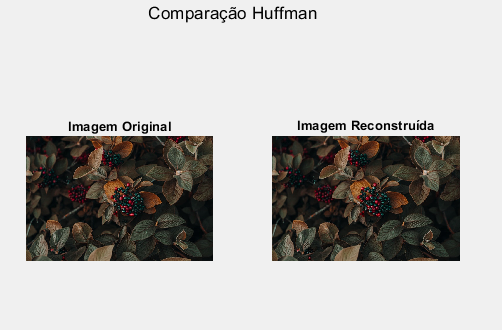
\includegraphics[width=\linewidth]{Captura de Tela (46).png}
  \caption{Legenda da Imagem 1}
\end{minipage}%
\begin{minipage}{0.5\textwidth}
  \centering
  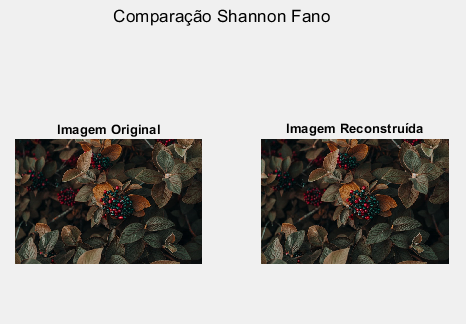
\includegraphics[width=\linewidth]{Captura de Tela (47).png}
  \caption{Legenda da Imagem 2}
\end{minipage}
\end{figure}


\section{Análises da tarefa}

De imediato, ressalto a dificuldade de processamento dos dados em termos de custos operacionais, refletido, por vezes, em consideráveis demoras nas respostas das etapas da tarefa, sendo muito custoso rodar o programa completo e analisar seus resultados de forma integral. Cito, também, que lidar com a codificação de imagens PNM usando as técnicas de Huffman e Shannon Fano mostrou ser uma tarefa que apresenta desafios significativos. 

Uma das primeiras dificuldades que enfrentei foi a necessidade de compreender suficientemente as técnicas de Huffman e Shannon Fano. Ambas envolvem conceitos complexos de codificação e decodificação, bem como a construção de dicionários. Esse entendimento requer tempo e estudo para entender basicamente como essas técnicas funcionam.

A implementação prática dessas técnicas também foi um ponto de destaque a ser comentado. Ela exigiu um certo conhecimento de programação e algoritmos, de modo que desenvolver o código para construir os dicionários, codificar e decodificar os dados não reforçam a ideia de que não se trata de uma tarefa trivial e requer habilidades de programação sólidas.

Além disso, as imagens PNM podem ter diferentes formatos, como PBM, PGM e PPM, cada um com suas próprias peculiaridades. Converter esses formatos em uma representação que possa ser tratada pelas técnicas de Huffman e Shannon Fano requer um entendimento aprofundado dos formatos de imagem e a capacidade de pré-processar os dados.

Outro desafio significativo foi a gestão da eficiência do código. Ao trabalhar com grandes volumes de dados, é fundamental otimizar o desempenho do código para evitar atrasos excessivos no processamento. Isso envolveu a implementação de estruturas de dados eficientes, como árvores de Huffman ou tabelas de frequência, para que a codificação e a decodificação fossem realizadas de maneira ágil.

Além disso, a adaptação das dimensões da imagem durante o processo de decodificação também se mostrou complexa. Como mencionado anteriormente, a discrepância nas dimensões entre a imagem original e a imagem decodificada exigiu soluções criativas, como o uso da função `imresize` no MATLAB, para garantir que a visualização final fosse precisa. Essa etapa de ajuste pode ser desafiadora, especialmente ao lidar com imagens de diferentes resoluções.

Outra dificuldade que encontrei está relacionada à necessidade de lidar com erros e exceções no código. Em situações reais, pode haver problemas na leitura, gravação ou decodificação dos dados, o que exige a implementação de tratamento de erros robusto para garantir a estabilidade do programa. Isso envolve a validação de entradas, verificação de integridade dos dados e a gestão adequada de exceções.

Por fim, a etapa de documentação e comunicação dos resultados também é um ponto importante a se considerar. Compreender e explicar as técnicas e o código desenvolvido para outros colegas ou para um público não técnico pode ser um desafio adicional. Portanto, a capacidade de traduzir conceitos complexos em termos compreensíveis para diferentes públicos é uma habilidade importante a ser desenvolvida.

Em resumo, lidar com a codificação de imagens PNM usando as técnicas de Huffman e Shannon Fano é uma tarefa desafiadora que envolve a compreensão profunda das técnicas, habilidades sólidas de programação, gerenciamento de eficiência, resolução de problemas e comunicação eficaz. Superar esses desafios requer tempo, dedicação e prática contínua.

Com relação à avaliação das taxas de compressão alcançadas na codificação de Huffman e Shannon-Fano aplicadas a imagens é importante para entender as vantagens e desvantagens desses métodos, considerando os diferentes tipos de imagens.

No caso da Codificação de Huffman, este método tem algumas vantagens significativas. Primeiramente, é altamente eficiente na compressão de dados discretos, como imagens em escala de cinza, onde cada pixel é tratado como um símbolo. A eficiência se deve ao fato de que Huffman atribui códigos mais curtos às ocorrências mais frequentes, economizando espaço quando as probabilidades são desiguais.

Além disso, a vantagem de Huffman inclui a simplicidade de sua implementação, o que torna a codificação e a decodificação relativamente rápidas, ajudando a otimizar o tempo de resposta do processo.

Entretanto, as desvantagens da codificação de Huffman podem ser observadas em imagens coloridas ou com padrões complexos. Nesses casos, a compressão pode não ser tão eficiente, pois as probabilidades de ocorrência dos símbolos podem se tornar mais equilibradas, resultando em códigos mais longos e, portanto, menos compressão.

No caso da Codificação de Shannon-Fano, suas vantagens incluem a capacidade de lidar com imagens mais complexas e coloridas de forma mais eficiente do que a codificação de Huffman. Shannon-Fano é mais adequado para situações em que as probabilidades dos símbolos são mais equilibradas.

No entanto, o Shannon-Fano pode ser menos eficiente do que Huffman em cenários onde as probabilidades são altamente desiguais, pois ele não necessariamente atribui códigos mais curtos às ocorrências mais frequentes. Além disso, a implementação do Shannon-Fano é mais complexa do que a de Huffman.

As taxas de compressão obtidas com ambos os métodos variarão dependendo do tipo de imagem. Em imagens simples em escala de cinza, a codificação de Huffman provavelmente oferecerá melhor compressão devido à sua eficiência nesse cenário. No entanto, em imagens coloridas ou com padrões mais complexos, o Shannon-Fano pode se destacar.
   
\bibliographystyle{alpha}
\bibliography{sample}
\begin{enumerate}
    \item 
    http://wiki.icmc.usp.br/images/0/0c/SCC0202-aula-13-Arvore\_Huffman.pdf
    \item https://www.ime.usp.br/~pf/analise\_de\_algoritmos/aulas/huffman.html
    \item https://pt.wikipedia.org/wiki/CodificaficaçãodeHuffman
    \item http://multimedia.ufp.pt/codecs/compressao-sem-perdas/codificacao-estatistica/algoritmo-de-huffman/
   \item https://github.com/ankmish/Encoding-in-MATLAB/blob/master/ShannonFano.m
\end{enumerate}
\end{document}